\chapter{Theory}
\label{ch:Theory}

In this chapter we introduce the theoretical background of \textit{citizen science} (\tracknshrink{CS}) and \textit{liquid democracy} (\tracknshrink{LD}). At first, in \autoref{sec:Theory_CS}, we define the term citizen science, provide examples to illustrate the concept and how to classify them. Likewise, in \autoref{sec:Liquid_Democracy}, we briefly recap on democracy and why representative democracy has flaws, that liquid democracy may address. We then explain how liquid democracy works. At the end of each section we provide a critical perspective of the corresponding concept.


% Clara
\section{Citizen Science}
\label{sec:Theory_CS}
\subsection{Background of Citizen Science}
\label{ssec:Background_CS}
Although Citizen Science in today’s academic world appears to be a rather contemporary term, the idea of citizens being involved in the scientific process dates way back. Taking, for instance, the \textit{Christmas Bird Count}; in 1900 the ornithologist Frank Chapman introduced the project---involving citizens in a yearly bird count---on Christmas Day. Starting with 27 participants the number of volunteers over the years has been growing significantly. Until today scientists use the accumulated longitudinal data of around 53 000 active members for large scale analyses that have been crucial for findings around population, distribution of species and migration etc. \parencite{Lebaron2017}. With modern technologies, the possibilities to involve citizens in the scientific process have become more various which consequently has led to a rapidly growing amount of Citizen Science projects. 

However, with increasing popularity, the term itself has become widely and rather differently used which makes it difficult to accurately define and differentiate it. Although the basic definition of involving members of the public in scientific research projects has remained, this definition leaves several questions open: Which sort of participation and to which extent the citizens are involved in a project? What defines a citizen and what does it need to qualify a citizen science project? In the past several years researchers have tried to define more systematically what citizen science means and what a \tracknshrink{CS} project can consist of. In the following, we will look at two  different theoretical perspectives on Citizen Science projects. 



\subsection{Types of Citizen Science Projects}
\label{ssec:Types_CS}
As mentioned before, the number of Citizen Science projects has expanded. Experience has shown that with thoughtful study design and under the right circumstances, Citizen Science can work on a massive scale, generating high-quality data that lead to reliable, valid scientific outcomes as well as unexpected insights and innovations  \parencite{Hakalay2014}. Therefore, more and more scientist involve Citizen Science in their research process. Though looking at various CS projects it quickly becomes  obvious that although they all involve some sort of citizen participation the projects themselves are quite different. \citeauthor{WigginsCrowston2011} have therefore created a typology, categorizing the projects into six different types. Examining common characteristics of 36 projects, grouping similar projects that share the same structure of participation, and some organizational as well as macro structural properties. The authors differentiate between action-, origination-, conversation-, investigation-, virtual- and educational projects. Looking at the different kinds of projects they also summarize scientific organizational as well as technology issues common with the different “modes” of Citizen Science \parencite{WigginsCrowston2011}. The following sections provide a brief overview on the different types of projects. 

\subsubsection{Action Based Projects}
Action-oriented projects generally encourage participants to intervene in local concerns, using scientific research methods as a tool to support civic agendas. In contrast to other types of initiatives, an action-orientated project materializes in form of a grassroots movement, as they are generally neither conceived nor planned by scientists. As an example, the \textit{Sherman’s Creek Conservation Association}, an organization with the goal to protect local creek and to provide environmental education. In action-based projects, so \citeauthor{WigginsCrowston2011}, researchers are often more consultants than collaborators. The, therefore, missing scientific method and spatial training generally prevent the collected data to become part of the scholarly knowledge base. The fact that these often are originated on a local level and is as well originated regarding local concerns cause the problem that there often lack funding and infrastructure which make it difficult for the project grow bigger than the original local level \parencite{WigginsCrowston2011}.

\subsubsection{Conservation Projects}
Conservation projects support stewardship and natural resource management goals, primarily in the area of ecology. Like Action projects, they are strongly rooted in local communes and volunteer engagement focuses on data collection activities, but in contrast to the Action projects, most conservation projects have affiliations with larger agencies.  Most projects include explicit educational goals or content. In regard to the scientific level, conservation projects often show a larger involvement of scientist, and projects without strong academic affiliations are typically lead by professional researchers employed in governmental organizations. From an organizational point of view, it is interesting to observe that conservational-oriented projects can be organized with top-down (researcher-initiated) as well as middle-out structures  (management-initiation)  \parencite[xx]{WigginsCrowston2011}.

\subsubsection{Investigation Projects}
Investigation projects are---in contrast to the conservational and action-based projects---focused on the scientific research goals which often consist of data collection. From this point of view, the Investigation project fits the other definitions of Citizen Science projects (\cite{Hakalay2014} \& \cite{Arnstein1969}). While education is not the foremost goal, some background material is often provided informing about the scientific background. Examples such as Great Sunflower\footnote{\url{https://www.greatsunflower.org/}} and FoldIt\footnote{\url{https://fold.it/portal/}} prove that this type of projects have the capability to engage thousands of participants, and to scale accordingly. Most Investigation projects involve or nonprofit conservation organizations as the primary organizers, and a top-down structure of organizing is a defining characteristic. Organizational issues appear with a fast growing number of participants as management and sustainability challenges grow accordingly. \parencite{WigginsCrowston2011}

\subsubsection{Education Projects}
As the name indicates the primary goal of Education projects is education and outreach. An exemplary project here is Fossil Finders\footnote{\url{http://fossilfinder.org/}}. The project is connecting educators, students as well as researchers to develop workshops primarily for schools. Because of the ‘classroom atmosphere’ and supervised inquiry-based format, this particular project permits on the one hand a close involvement of the participants into the scientific process and on the other hand it also facilitates the expansion and extension of the project activities, such as collection, identification, and description of additional fossils. Nevertheless, the emphasis on education projects lies in the educational aspect while scientific contribution is of secondary importance. Additionally, the relative cost of acquiring data through education projects is substantially higher. All the above often end in education projects only being considered as a Citizen Science project only by the presence of including an academic institution or researcher as an organizer. Proceeding to the organizational issues, it is hardly surprising that all of the mentioned sample projects are top-down organized. Involving multiple partners the examined project all have substantial funding \parencite[xx]{WigginsCrowston2011}.

\subsubsection{Virtual Projects}
In contrast to all other project types described above, virtual projects are completely ICT-mediated with no physical element whatsoever. The exclusively virtual -based project shares its goal with investigation projects as its main focus is the scientific research often in form of data collection. While examples of these projects are numerous, for example: Galaxy Zoo\footnote{\url{https://www.zooniverse.org/}}, Whale FM\footnote{\url{https://whale.fm/}} and Planet hunter\footnote{\url{https://blog.planethunters.org/}}, the line to projects that not further fall under the definition to Citizen Science is narrow. Whether Citizen Science is defined as citizen participation or includes an active involvement of its members, virtual projects often run danger to not match the definition of a citizen science project \parencite{Hakalay2014}. As for investigation projects, the primary challenge for virtual projects is ensuring valid scientific results. This matter is complicated by the fact that it is rather difficult to maintain the volunteers’ interests. Even though motivation concerns are often addressed by game-like task design, it is often difficult to collect valid data. Many virtual projects compensate the missing quality of the data by providing a quantity of tasks. Nevertheless, this problematic is worth keeping in mind. Looking at the organization of virtual projects, \citeauthor{WigginsCrowston2011} conclude that all of their examined projects are top-down organized and exclusively run by academics. Consequently, the projects are most and foremost financed by research funding and shareholders what often poses a threat to the project’s sustainability. \parencite{WigginsCrowston2011}

\subsection{Haklay’s Ladder of Participation}
\label{ssec:Ladder_Participation_CS}

The extent to which volunteers are involved in a Citizen Science project plays a crucial part regarding the nature of the project. To qualify as a Citizen Science project the non-professional scientists must take an active role in the research process \parencite{Eitzeletal2017}. This “active” role, however, ranges form discovering objects in pictures (like in Galaxy Zoo) to finding, describing and identifying actual Fossils\footnote{\url{http://fossilfinder.org/}}. To closer define this rather large spectrum of participation \citeauthor{Hakalay2014} introduces the \textit{Ladder of Participation} distinguishing between four different levels of involvement. At the most basic level, participation is limited to the provision of data/resources and minimal cognitive engagement. Hacklay titles this level of participation \textit{Crowd Sourcing} as volunteers often barely function as better sensors \parencite[xx]{Hakalay2014}.

The next level is the so-called \textit{Distributed Intelligence}. Here the cognitive ability of the participants is crucial. Many Citizen Science projects operate on this level. Volunteers are needed to take some basic training to collect data or carry out simple interpretation activity. On this level of engagement volunteers with time can learn more about the topic and advance beyond their initial training and be given more advanced tasks \parencite[xx]{Hakalay2014}.

What distinguishes the next level \textit{Participatory Science} is that the volunteers are involved not only in the data collection but in the problem definition. In the above mentioned Fossil Finders project the participants are not only engaged in data collection but also---with assistance of experts---taking part in the analysis and interpretation of the results. Participants can suggest research question, which than can be explored with the data collected \parencite[xx]{Hakalay2014}.

The last and highest level on the ladder is the level of \textit{Collaborative Science}. Here the participants can choose their level of engagement and can be potentially involved in analysis, publication or utilization of the results. Scientists, in addition to their role as experts, function as facilitators. \citeauthor{Hakalay2014} states, that this mode of Citizen Science even opens the possibility of Citizen Science without professional scientists \parencite[xx]{Hakalay2014}.

\citeauthor{Hakalay2014} summarizes, that one project not necessarily have to be classified in only one category. Seeing for example the volunteer computing projects. While most participants will start  at the bottom level, collecting data or carrying out basic interpretation, some volunteers  might move to the second level assisting or teaching other volunteers, or even  communicate with the scientists, discussing results or suggest new research directions \parencite[xx]{Hakalay2014}. \citeauthor{Hakalay2014} concludes that participation in Citizen Science can take different forms, while in some projects the gap between professional scientist and participants is wider, other projects facilitate collaboration, teaching volunteers so that they become more involved in the scientific process altogether.

\subsection{Issues and Open Questions}
\label{sec:Issues_CS}

\citeauthor{WigginsCrowston2011} and \citeauthor{Hakalay2014} agree, that the number, as well as the diversity of Citizen Science projects, are vast. Nevertheless, the objective to include citizens in the scientific process itself sometimes seems to be at the very core of the project and other times more of a side effect. It also appears that even though the number of Citizen Science projects is growing, the data is still used cautiously in papers and scientific publications \parencite[xx]{Hakalay2014}. Especially for projects in which the influence of scientist is relatively small. \citeauthor[xx]{FlanaginMetzger2008} state that this might be due to the fact that many researchers still mistrust the quality of the data produced by citizens. While \citeauthor[xx]{Holling1998} emphasized that there are two cultures of science and that Citizen Science by necessity belongs to the type of science that incorporates uncertainty and highlights integrative approaches \parencite[xx]{Holling1998}

Another question left open is what exactly defines a Citizen and what a Scientist. Through the preceding text, we deliberately have left this question open since Citizen Science itself questions---to some extent---the classic definition of Science as well. Defining a scientist as someone being employed to carry out scientific work or research the differentiation stays rather clear. But as soon as it comes to unpaid scientists the situation is far more complex. It would mean to define scientists throughout their way of working with scientific frameworks, data collection, and interpretation as well as their overview and knowledge about the field, being able to place the newly retrieved information in the already existing body of work. Nevertheless, pursuing this definition a well-trained and informed citizen could then also meet these criteria. Authors like \citeauthor{StilgoeLockWilsdon_2014} and \citeauthor{Irwin1995} take this thought process one step further declaring that changing the epistemology of science could be seen as one goal of Citizen Science. They advocate that on a “extreme” level of Citizen Science the emphasis shouldn´t be on the citizen as a scientist but the scientist as a citizen. Meaning that in some cases it shouldn’t be possible to draw the line between Scientist and Citizen. However, \citeauthor{Irwin1995} also notes that this way of conceptualizing and practicing science is not widely accepted in the current culture of science. \parencite[xx]{Irwin1995}


\section{Liquid Democracy}
\label{sec:Liquid_Democracy}

\subsection{Democracy Recap}
\label{ssec:Democracy-Recap}

Even though there are many forms of political government, it is democracy that spread around the globe over the last hundred years (see \autoref{fig:democracy-trend}). \textit{“As of the end of 2016, 97 out of 167 countries (58\,\%) [\ldots] were democracies [\ldots]”} \parencite{Desilver2017}. According to the observations in \autoref{fig:democracy-trend} it can be argued that democracy is a successful and thus modern structure, since there is no competing political system showing a similar thriving trend as democracy does. It is, however, important to mention that there are concerns about the recent ‘health status’ of democracies. As an reputable example, \textit{Freedom House}---an U.S. government-funded \tracknshrink{NGO}---states in their current annual report series: \textit{“In 2018, Freedom in the World recorded the 13th consecutive year of decline in global freedom\footnote{\textit{Freedom House} measures \textit{freedom} with a score rating various democratic characteristics of a country. Thus, an undemocratic country scores ultimately lower.}.”} (see \cite{FreedomHouse2019}). On the other hand, using the same data by \textit{Freedom House}, yet on a much larger timescale (1973 to 2014), it reveals a positive trend towards the amount of free and partly-free countries\footnote{The English Wikipedia plotted these data: \url{https://en.wikipedia.org/wiki/Freedom_in_the_World\#Trends}}. Therefore it is important to evaluate such data on time frames lasting over decades and centuries as \autoref{fig:democracy-trend} does. 

\begin{figure}[H]

	\centering \begin{tikzpicture}
	\node[anchor=south west,inner sep=0] (image) at (0,0,0) {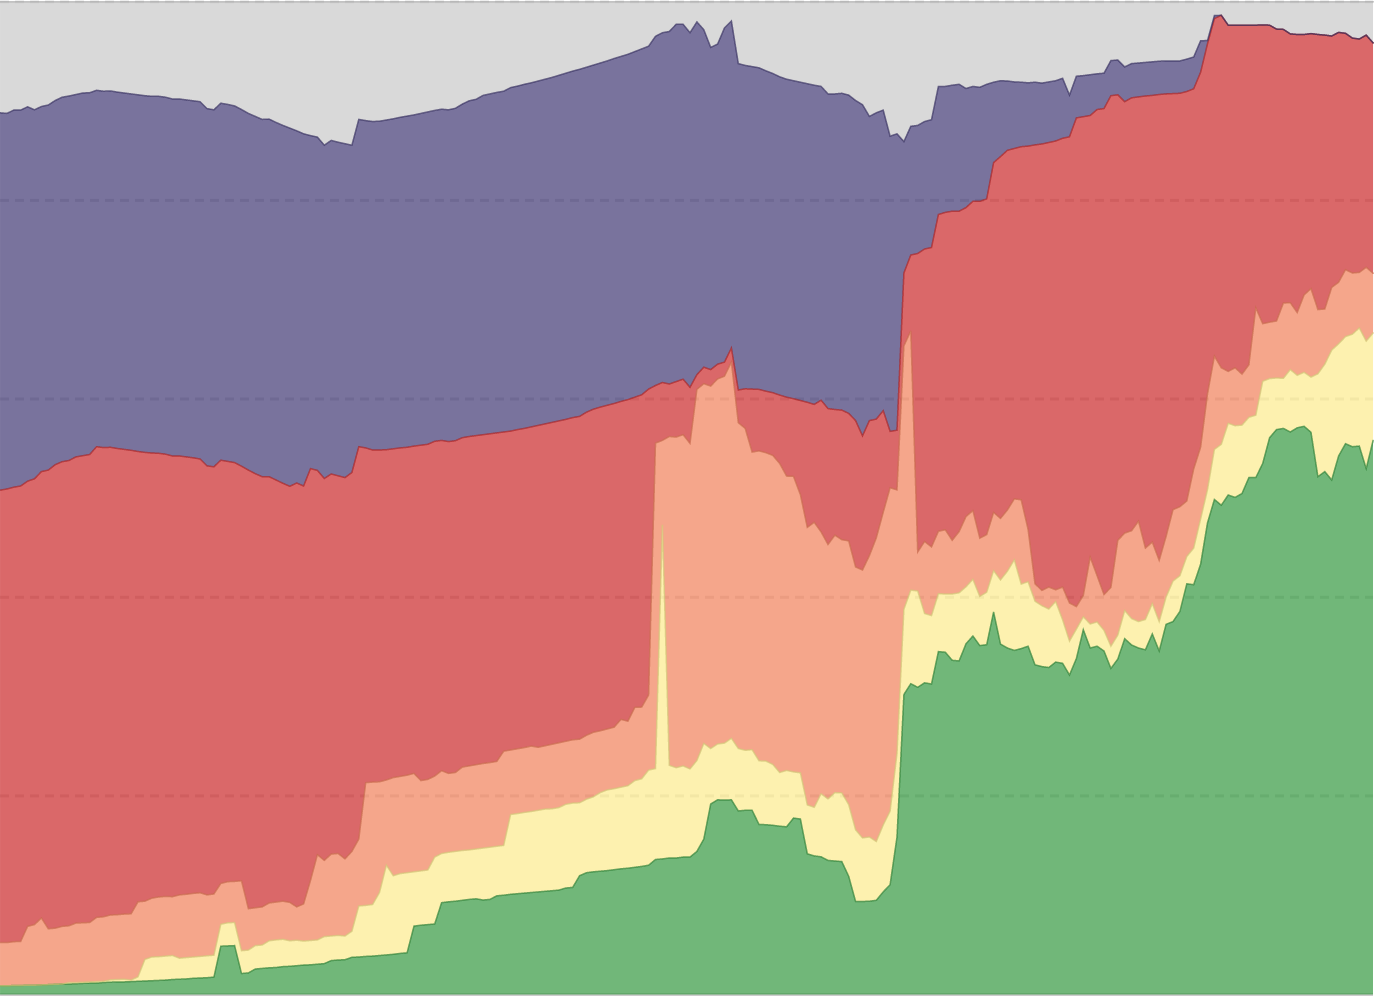
\includegraphics[width=8cm]{democracy-trend.png}};
	\begin{scope}[x={(image.south east)},y={(image.north west)}]
% 	% next four lines will help you to locate the point needed by forming a grid. comment these four lines in the final picture.↓
% 		\draw[help lines,xstep=.1,ystep=.1] (0,0) grid (1,1);
% 		\draw[help lines,xstep=.05,ystep=.05] (0,0) grid (1,1);
% 		\foreach \x in {0,1,...,9} { \node [anchor=north] at (\x/10,0) {0.\x}; }
% 		\foreach \y in {0,1,...,9} { \node [anchor=east] at (0,\y/10) {0.\y};}
% 	% upto here↑
    
	\libertineLF
	\draw (-0.05,0.0) node {\small{0\,\%}};
    \draw (-0.06,0.2) node {\small{20\,\%}};
    \draw (-0.06,0.4) node {\small{40\,\%}};
    \draw (-0.06,0.6) node {\small{60\,\%}};
    \draw (-0.06,0.8) node {\small{80\,\%}};
    \draw (-0.07,1.0) node {\small{100\,\%}};
   	\libertineOsF
    \draw (0.0,-0.06) node {1816};
    \draw (0.17,-0.06) node {1850};
    \draw (0.425,-0.06) node {1900};
    \draw (0.67,-0.06) node {1950};
    \draw (0.93,-0.06) node {2000};
    
	\draw[-latex] (0.99,0.25) -- +(0.5cm,0cm)node[anchor=west] {\scriptsize{Democracy}};
    \draw[-latex] (0.99,0.6) -- +(0.5cm,0cm)node[anchor=west] {\scriptsize{Open Anocracy}};
    \draw[-latex] (0.99,0.695) -- +(0.5cm,0cm)node[anchor=west] {\scriptsize{Closed Anocracy}};
    \draw[-latex] (0.99,0.85) -- +(0.5cm,0cm)node[anchor=west] {\scriptsize{Autocracy}};
    \draw[-latex] (0.99,0.96) -- +(0.5cm,-0.28cm)node[anchor=west] {\scriptsize{Colony}};
    \draw[-latex] (0.99,0.98) -- +(0.5cm,0cm)node[anchor=west] {\scriptsize{Transition/No data}};

	
	\end{scope}
	\end{tikzpicture}
	\caption[World population by political regime]{World population by political regime \parencite[see][]{Roser2018}.}
	\label{fig:democracy-trend}

\end{figure}

It is, however, neither within the scope of this project report to asses democratic trends, nor other systems of rule. Democracy, however, entails various advantages compared to other political systems. First and foremost---by its literal translation\footnote{\textit{Rule of the people}, from Ancient Greek: \textgreek{Δημοκρατία} (Dēmokratía): democracy, whereby \textgreek{Δῆμος} (Dêmos) means \textit{the people}, and \textgreek{Κράτος} (Krátos) means \textit{power/strength}.}---democracy empowers its citizens to participate in political processes, and therefore to influence the political pathway. For example, one fundamental element is suffrage, that is, the right to vote. Additionally, democracy allows its people to shape the system’s frame. Thus, a wide range of democracy types\footnote{For further reading see the Wikipedia article \textit{Types of democracy}: \url{https://en.wikipedia.org/wiki/Types_of_democracy}.} have evolved over time.

The two most prominent types of democracy are direct and indirect (or representative) democracy. In direct democracy citizens are directly involved in the decision-making of the state, which is, however, only feasible for smaller populations. Since direct democracies do not scale for growing communities, it is impossible to inform every citizen “\textit{[\textellipsis{}] about all issues as they either do not have the time, the desire or the expertise.}” \parencite{Schiener2015}. On the other hand, representative democracies---where elected officials represent the voters---scale well, but fail to serve the citizens’ interests. \citeauthor{Schiener2015} summarizes three main flaws for representative democracies: (1) “\textit{[\ldots] citizens are limited to vote representatives of a restricted set of candidates [\ldots]}” and therefore “\textit{[\ldots] voters are forced to give up their personal preference and instead have to vote for the candidate with the highest prospects of being elected.}” (2) Since, representatives are limited in their accountability during and after their term in office, it is convenient to

\begin{displayquote}
“[\ldots] convince voters before an upcoming election of one’s competence by either introducing new proposals that are favored by the community (but most likely won’t be introduced), or by handing out expensive “Wahlgeschenke” (pre-election presents).”\\[1mm]
\hspace*{\fill}\textcite{Schiener2015}
\end{displayquote}

Lastly, representative democracies are vulnerable towards corruption due to a concentration of power. This may lead to a fraternization of politics and industry, in such forms as bribery and lobbying. In this report we focus on \textit{liquid democracy}, a variant of democracy that is also known as \textit{delegative democracy}, which is potentially able to tackle these three named concerns about representative democracy.


\subsection{Liquid Democracy Terminology}
\label{ssec:Liquid_Democracy}

Liquid Democracy (\tracknshrink{LD}) is a type of democracy lying in between two major democracy forms: direct democracy and indirect (or representative) democracy. This \textit{liquid} intersection allows citizens to either delegate their vote to a proxy (i.e., a representative) or to vote directly for a certain state of affairs (e.g., a proposition).

It is important to point out that the voting form \textit{proxy voting} shares some similarities of liquid democracy. There is, however, a fundamental difference: in liquid democracy a proxy may further delegate his/her voices to another proxy, which is not intended for proxy voting. Therefore, a proxy or representative, in the concept of liquid democracy, can be---mathematically---interpreted as a transitive (recursive) vertex within a directed graph. \citeauthor{Kahng2018} states:

\begin{displayquote}
“In contrast to the classic proxy voting paradigm \parencite{Miller1969}, the key innovation underlying liquid democracy is that proxies [\textellipsis] may delegate their own vote to a proxy, and, in doing so, further delegate all the votes entrusted to them. Put another way [\textellipsis] votes may freely flow through the directed delegation graph until they reach a sink.”\\[1mm]
\hspace*{\fill}\textcite{Kahng2018}
\end{displayquote}

The delegation graph is a fundamental component of liquid democracy. \autoref{fig:Delegation-Cascade} visualizes such a delegation graph/cascade. 

\begin{figure}[H]
\centering
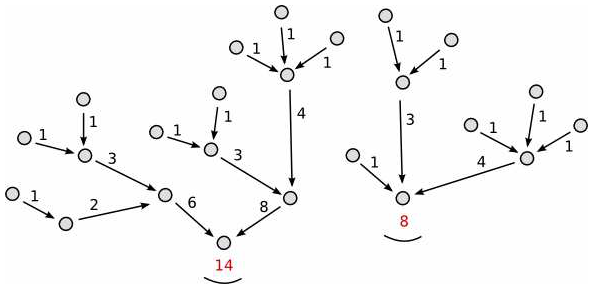
\includegraphics{delegation-cascade.png}
	\caption[Delegate cascade voting]{“A snapshot of a small election in which two separate cascades have formed. Vote flow is depicted by arrows, and volume by numbers. The votes flow together until they pool at the bottom, where they are held by the leading candidates.” \parencite{Allen2008}}
	\label{fig:Delegation-Cascade}
\end{figure}
However, direct voting is neither intended in proxy voting nor in delegation graphs. Therefore---and to fulfill the initial definition of \tracknshrink{LD}---the delegation graph must be extended to permit direct voting, which then allows to further classify the terms: proxy voting, delegation graph and liquid democracy in a true subset relationship: \textit{proxy voting \(\subsetneq\) delegation graph \(\subsetneq\) liquid democracy}. Thus, the concept of liquid democracy acts as a superset for proxy voting and delegation graphs. 

\subsection{Liquid Democracy Mechanics}
\label{ssec:Liquid_Democracy_Mechanics}

Due to its superset position liquid democracy combines characteristics from proxy voting, delegation graphs and direct voting. To visualize this concept in a simplified manner \autoref{fig:Liquid-Democracy-Delegated-Voting} illustrates the main steps of a voting process within a liquid democracy system.

In liquid democracy, and in directed delegation graphs, the vote always flows from a \textit{principal} to a \textit{proxy}, and, initially, each citizen always starts as a  principal holding their own voice, as depicted in the first column in \autoref{fig:Liquid-Democracy-Delegated-Voting}. From there, each individual has two choices: (1) to vote \textit{directly} for a given state of affairs (Option A, B or C) or (2) to \textit{delegate} their voice to a proxy. Naturally, and for the sake of completeness, citizens have the right to abstain from voting at all, however, in this work we set the focus on people seeking for participation. Thus, choice (1) entitles citizens to \textit{directly} influence a given state of affairs, as depicted in red. Apparently, voting as a ‘initial principal’ yields to the lowest voting impact of \(1\), which is by definition your own inherent voice. Choice (2) entitles citizens to \textit{delegate} their voice to a proxy, which can be the case when the (initial) principal is doubtful in their decision-making (\textit{uncertainty} is depicted by gray color in \autoref{fig:Liquid-Democracy-Delegated-Voting}).

If, however, an individual receives a single voice or multiple voices they automatically become a proxy. In this position they have the same two choices as the principals had before, that is, to either directly vote or to further delegate their votes. This characteristic demonstrates the recursive nature of a liquid democracy system. In the case of an uncertain proxy (column two, \autoref{fig:Liquid-Democracy-Delegated-Voting}), the proxy might further delegate their voices. Technically, by doing so, the proxy becomes a principal, yet with a higher voting impact, since the voting count gets accumulated along the graph, whereby each node has a natural weight of \(1\).

Ultimately, each edge will hit at some point their last node, which are---in a liquid democracy system---individuals being certain about their decision-making and have an opinion (\textit{certainty} is depicted by colors in \autoref{fig:Liquid-Democracy-Delegated-Voting}). In this step there are no further delegations.

\begin{figure}[H]
	\centering \begin{tikzpicture}
	\node[anchor=south west,inner sep=0] (image) at (0,0,0) {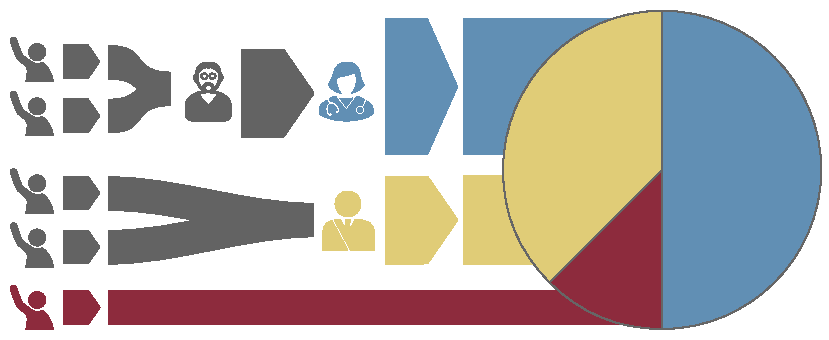
\includegraphics[width=\linewidth]{Liquid-Democracy-Delegated-Voting.pdf}};
	\begin{scope}[x={(image.south east)},y={(image.north west)}]
% 	% next four lines will help you to locate the point needed by forming a grid. comment these four lines in the final picture.↓
% 		\draw[help lines,xstep=.1,ystep=.1] (0,0) grid (1,1);
% 		\draw[help lines,xstep=.05,ystep=.05] (0,0) grid (1,1);
% 		\foreach \x in {0,1,...,9} { \node [anchor=north] at (\x/10,0) {0.\x}; }
% 		\foreach \y in {0,1,...,9} { \node [anchor=east] at (0,\y/10) {0.\y};}
% 	% upto here↑
    
    \draw (0.045,1.03) node {\textsf{\textbf{Principal}}};
    \draw (0.250,1.03) node {\textsf{\textbf{Proxy 1}}};
    \draw (0.415,1.03) node {\textsf{\textbf{Proxy n}}};
    \draw (0.580,1.03) node {\textsf{\textbf{Option}}};
    \draw (0.800,1.03) node {\textsf{\textbf{Results}}};
    
    \draw[line width=0.1mm] (0,0.992) -- (0.98,0.992);
    
    \draw (0.068,0.730) node {\textcolor{gray}{\(\textsf{\footnotesize{1}}\)}};
    \draw (0.068,0.571) node {\textcolor{gray}{\(\textsf{\footnotesize{1}}\)}};
    \draw (0.068,0.353) node {\textcolor{gray}{\(\textsf{\footnotesize{1}}\)}};
    \draw (0.068,0.193) node {\textcolor{gray}{\(\textsf{\footnotesize{1}}\)}};
    \draw (0.068,0.002) node {\textcolor{gray}{\(\textsf{\footnotesize{1}}\)}};
    
    \draw (0.280,0.618) node {\textcolor{gray}{\(\textsf{\footnotesize{3}}\)}};
    \draw (0.450,0.618) node {\textcolor{gray}{\(\textsf{\footnotesize{4}}\)}};
    \draw (0.450,0.232) node {\textcolor{gray}{\(\textsf{\footnotesize{3}}\)}};
    
    \draw (0.58,0.74) node {\textsf{\textcolor{white}{\textbf{A}}}};
    \draw (0.58,0.35) node {\textsf{\textcolor{white}{\textbf{B}}}};
    \draw (0.58,0.10) node {\textsf{\textcolor{white}{\textbf{C}}}};
	
	\end{scope}
	\end{tikzpicture}
    \caption[Illustration of liquid democracy]{Illustration of a liquid democracy system. Each individual has a voice, depicted by the numbers. Citizens may either vote directly or delegate their voice. Delegation will accumulate the voice impact for a proxy. Certainty is color-coded, whereas uncertainty is gray-coded.\\
    \hspace*{\fill}
    \scriptsize{\textit{Icons provided by thenounproject.com under Creative Commons 
\includegraphics[height=\fontcharht\font`\X]{cc-icon.pdf} license}}\\
    \hspace*{\fill}
    \tiny{\textit{
    	\url{https://thenounproject.com/icon/575955/}, 
    	\url{https://thenounproject.com/icon/24402/},\\
    	\hspace*{\fill}
        \url{https://thenounproject.com/icon/751412/}, 				\url{https://thenounproject.com/icon/1471169/}
        }}
	\label{fig:Liquid-Democracy-Delegated-Voting}}
\end{figure}

\subsection{Critical Perspective}
\label{ssec:LD-Critical-Perspective}


In a representative democracy citizens entrust their voice---in accordance to their own mindset---to a certain proxy who is, usually, better-informed. However, if the proxy is uninformed for a certain state for affairs it is not possible to further delegate the received votes. This ultimately results in damaging or unsustainable decisions made by the proxy. This phenomenon is related to the \textit{Peter principle} by \textcite{Peter1969}, that means: “\textit{In a hierarchy every employee tends to rise to his level of incompetence.}”. Thus, in a liquid democracy this would be unlikely to happen since, in theory, the vote flows always to better informed citizens. This concentration flow, however, can bear the risk for abusive behavior. Users could pretend to have a certain expertise by well-promoted marketing about their persona, so they could `collect' voices and use them for either their own interest or other’s (e.g., corporate) interests. It is also questionable if people would delegate at all, or rather vote most of time directly without knowing the field very well and being unaware about the consequences. \textcite{Bargmann2017} states that ``\textit{[\textellipsis{}] giving ordinary people more power who may not fully understand the ramifications of their vote could be disastrous for the running of a country.}''


Additionally, a fundamental requirement for digital liquid democracy platform is a solid digital infrastructure. This should be granted for every citizen, since a lack of access to such a platform would mean a withdraw of the voice of a citizen. 

\todo[inline]{Mention that vote anonymity is a crucial part}


Traditionally, in a parliamentarian democracy, the right to initiate and vote on propositions is exclusive for members of the parliament.
However, in a liquid democracy, by definition every participant has the right to vote on propositions, and participate in their constitutive phase.
Consequently, every participant should also have the unrestrained right to create propositions. This can also be abused be creating spam propositions. A platform should thus, also have protections mechanisms.


\subsection{Digital Liquid Democracy}
\label{ssec:Digital_LD}
While both direct democracy and representative democracy have existed before the digital revolution, and have thus been practiced before the availability of digital tools, digitalization has an enormous effect on liquid democracy. Although digitalization is often quoted for optimization, its true potential lies in its disruptiveness, which means that---as a game changer---digitalization enables processes that would not be possible otherwise. These two perspectives on digitalization are caught exemplary by the blog entry of \textcite{Veuve2015}, which focuses on process efficiency and mentions that liquid democracy and digitalization can raise the number of participants in political process, but also remarks on the dedogmafication\footnote{That is the development of politics to be less based on dogma, i.e. fundamental principles or doctrines, strong, indisputable believe, established opinions or code of tenets}  of politics. This dedogmafication implies that representative democracy is becoming an anacronism, and that digitalization has the disruptive potential to reform this form of governance towards liquid democracy. 

\textcite{Bargmann2017} views it the other way around, as digitalization being the requirement for implementing the complex voting procedures for liquid democracy. This would be impossible to perform offline. 
The popularity of online propositions coincides with the observation of political apathy, which shows the need for more participatory opportunities in the political sphere. In a representative democracy, participation is limited to propositions (which rarely have any real effect), professional politicians (which is not a real option for most citizens) or activities out of the direct sphere of politics (in the form of social activism). This lack of participatory opportunities is seen as the problem of liquidity (as the lack of availability of resources to bring about political change) by the \href{https://www.democracy.earth/}{democracy.earth} project. This lack is ever more obvious in the decline of freedom within democracies and political apathy of voters, which they see as a problem of liquidity of these systems (\href{https://govfresh.com/2019/01/liquid-democracy-blockchains-and-governance-in-the-post-nation-state-era/}{id.}). While formally the political system of democracy is on the win (as shown in \autoref{fig:democracy-trend}), the rise of autocratic tendencies\footnote{as seen for example in the \href{https://freedomhouse.org/report/freedom-world/freedom-world-2019/democracy-in-retreat}{Freedom In the World reports}} is not unlikely to stem from a crisis of political liquidity.

With the shift from passive consumers to active participants through the Web 2.0, as isolated within social bubbles it may be, digitalization has a participatory drive for societal processes. Coupled with the availability of knowledge and its universality of access, digitalization supports ease of discourse. This discourse can lead to anything from political impulses to revolutions. The knowledge stemming from these processes and `crowd intelligence' is too precious not to be used for systems that give sovereignty to their citizens. Even more so, \textcite{Jonsdottir2015} warns that wisdom needs to be extracted from this knowledge.
The increasing interconnectivity through technology, processes and interaction has the potential to make the individual more vulnerable, but allows for organization, informedness and control. This, however, requires participatory political structures and processes, which are just the fundamentals that liquid democracy addresses.


\section{An Integrative Perspective for Citizen Science in Liquid Democracy}
\label{sec:Integration_CSLD}
The arguments above show that liquid democracy, in particular in a digitalized age, has the potential to be a powerful vehicle for the empowerment of citizens as political subjects. Where citizen science strives for the scientific and educational empowerment of citizens, liquid democracy aims at their political empowerment. The discussion furthermore implies that the quality of the political discourse depends on a sound factual basis of digital liquid democracy and the informedness of political subjects. This is particularly the case for a society challenged and blessed with interconnectivity. It requires the shift of power structures from representational politics, that is solely confined to professional politicians and rigid parties, to 'the (informed) masses'; similarly, in the current system, science is strongly confined to professional scientists and institutions instead of the broad masses. Both, the concept of citizen science and liquid democracy thus address a shift of power from exclusive spheres within the society to empowerment of citizens. That does not mean that either program wants to do away with the professional practitioner. On the contrary, both require highly competent, capable and trained professionals that, in addition to their own specialty, have profound transdisciplinary skills that give them the responsibility for a professional perspective on the issues at hand.


The heterogeneity of actors involved both in scientific processes (or more generally said in processes of knowledge generation and construction) and in political processes is of paramount value, not only for the constructed matter to be comprehensible for broad swathes of society, but for the organization of the process itself. This hetereogeneity is not only what democracy is based upon, but also makes research richer and broadens the scientific discourse.


Citizen science and liquid democracy may contribute to each other: a citizen science project may fetch the huge amount of data---generated by a liquid democracy platform---and citizens may then analyse a wide field of topics, formulate and test hypothesis. With this gained insight citizen science may also be able to further shape a liquid democracy platform. Depending on the amount and type of data which can be accessed by citizens, potentially all levels in \citeauthor{Hakalay2014}’s framework (\citeyear{Hakalay2014}) may be covered.

The participation of citizens is not limited to the production of their own data (i.e., by votings, delegations, takings polls etc.); it also extends the political discourse through speeches, discussions, propositions, etc. Instead, going beyond crowd sourcing, the analysis, comprehension and feedback of the core data of the political processes is a fundamental element of participation and involvement in the political process in a mature democracy. This is particularly true since political data is self-referential, in the sense that political data and processes refer to political data and processes themselves, and analyses and opinions are subject to political processes as well.

In addition to the generation and analysis of data, liquid democracy can provide a laboratory for developing and testing hypotheses. Since in \tracknshrink{LD} the researcher and the subject of investigation fall together, they can act on the matter they analyze, by actively participating in the discourse with an agenda (albeit a scientific agenda instead of a political agenda), and by observing the process of the agenda unfolding. While the pursuit of a scientific goal requires some discipline of the researcher (who as a political subject often has the impulse to pursue political goals at the same time, which they need to curb in the interest of science), the strong influence of the research on the analyzed matter, makes this a very favorable subject (at least within the social sciences, where researchers often have to work from a purely observational point instead of being able to control the system of investigation). 

Through the inclusion of citizens in all steps of the scientific process\footnote{it goes without saying that citizens can also be included in the dissemination and publishing of the scientific results}, (digital) liquid democracy can provide a favorable subject for citizen science. Providing the means, in particular the tools, support and training for their inclusion is the biggest challenge for citizen science. Aiming at a high level within the framework of \textcite{Hakalay2014} requires the provision of a sound structure for conveying the scientific method and necessary skills, as well as counseling. A more concrete and in-depth analysis of this requires a through analysis of all steps of the scientific process (with a regard to the particularities of the methods and idiosyncrasies of the field and subject), for the analysis of the involvement of citizens within the scientific process. Training of citizens is of utmost importance. This involves the provision of tools, workshops, training session etc. 

Moreover, a healthy political discourse needs a sound factual and scientific basis; in particular one that can be understood by political subjects. By opening up the analysis of political issues and processes to citizen scientists, the system of impartial information stemming from political and social scientists, journalists, \tracknshrink{NGO}s and political commentators and analysts can be enriched by another group of actors: empowered political subjects themselves. Furthermore, by including political subjects in the process of deriving knowledge, the educative element of citizen science is strengthened, so that they can make more informed decisions. This may also alleviate political apathy of the citizens involved in these projects, although it is likely that most citizens involved in \tracknshrink{CS} projects on political matters are not predisposed to political apathy to begin with.

As discussed above, citizen science is often accused of amateurism\footnote{Which is to a large extend the whole point of citizen science.}, which may be a valid point of critique to some extend, especially when the projects are poorly set up. For the political discourse, however, the matter is somewhat different. Political discourse is (or should be) often based in (established) science. However, methods within an active political discourse are much less strict than those used in science, and the role of rhetorics and agenda-setting are more important than the epistemological state of its statements. The political discourse is less exclusive than scientific discourses, and political skill and the formation of policies can be seen as influencing the dynamics of opinions in groups.

As stated above, both (digital) liquid democracy and citizen science can contribute a lot to one another, and different synergies exist between the two. However, the concepts do not have a symmetric relation to one another; in a simplified way one could say that one is the matter and the other one is the method. Citizen science methods are to some degree institution-dependent, and even more general work is always strongly focused on particular projects. Thus, our priority lies in the analysis of liquid democracy rather than citizen science.

One large problematic matter, however, for bringing together citizen science and liquid democracy remains: the issue of privacy and open data, which will be discussed in the following.


\subsection{Data Accessibility and Anonymity}
\label{ssec:Integration_AccessibilityAnonymity}

Arguably the most challenging aspect of a \tracknshrink{CS}-enabled \tracknshrink{LD} platform, is the tension between data accessibility and anonymity. As stressed in \ref{ssec:LD-Critical-Perspective} (\nameref{ssec:LD-Critical-Perspective}), vote anonymity is a crucial aspect of democratic voting systems. Yet, if data accessibility is too restriced the citizen scientist degrades to a data provider. Since by suppressing the system’s participatory nature it would be transformed into a mere crowd-sourcing platform (from a \tracknshrink{CS} perspective). For allowing citizens to pose (and investigate) research questions based on real-world data within their context of interest and expertise, as well as for principal\footnote{Political actors that delegate their votes to another actor.} to evaluate whether their values are represented appropriately by proxies\footnote{The political actor that principals delegate their vote to.}, data accessibility / transparency (at least to some degree) is imperative.

Although at first glance transparency and anonymity might seems like a zero-sum game where increased data accessibility constitute a violation of a user’s privacy, a number of strategies do exists that tackle these problems. With proper encryption techniques, such as homologous encryption, these problem might be solved, since required operations could be performed wile preserving user anonymity; However, no appropriate operators exist for this problem, and which information can be derived by whom would still be an issue that needs to be tackled by security-by-design; prohibiting users from deriving knowledge (that could be used to infer aspects of the persona) is against the point of \tracknshrink{CS}.

\subsubsection{Decoupling User Accounts from Personal Identity}

The most obvious strategy might be to decouple the user account (i.e., the digital identity) from the user’s personal identity. When done with proper protection and when the personal identity of the user is used solely to validate the vote connected to the account (or even only for the verification of the account), it can be argued that all data of the user can be transparent for everyone, and no restrictions on the data accessibility needs to be enforced. While this is the optimal solution from the perspective of the citizen scientist and the principal---who can (in theory) perfectly evaluate whether her political power was used as intended---this approach is not without danger. First and most obvious, when a breach of the separation of the user and personal identity of the user occurs. Perfect safety does not exist and many cases where highly sensitive information was exposed do exist\footnote{\url{https://www.msspalert.com/cybersecurity-markets/americas/voter-registrations-stolen/}}\textsuperscript{,}\footnote{\url{https://www.scmp.com/news/hong-kong/politics/article/2082566/laptops-containing-37-million-hong-kong-voters-data-stolen}}. One could also gain access to someone’s personal identity, indirectly. With more detailed data provided, profiles can be constructed which are more likely to be bound to a person by tying their digital persona to their personal identity. While this might be somewhat harder for non-public figures, for people active in the public sphere---by their personal identities (e.g., politicians)---this link would be easy to establish. One thoughtlessly given detail might be enough to link the entirety of the user persona to the human behind their account, making transparent in all activity and views every uttered on the platform. 
Most problematic about this issue from a participatory democratic perspective is the mechanics that more involvement leads to a higher probability of the user persona being linked to the person behind this, thus rather discouraging than encouraging engagement in the participatory processes.

\subsubsection{Aggregating User Data}

Another, rather conservative, solution for making user data anonymous is by aggregating voting behavior by demographic aspects of users. By clustering users according to their distinct demographic characteristics, statements about this group can be derived. This approach rests on the assumption that explanatory variables for political behavior are consistent among the chosen demographic aspects. In this way, researchers could derive meaningful statements about homogeneous groups of actors with similar cognitions and attitudes, while simultaneously preserving the anonymity and privacy integrity of the person behind a user.
A scientist would thus get access to the distribution of voting patterns, vote delegation patterns or involvement in issues by certain demographics. 

While seeming elegant at first, this method has two shortcomings. First, this employs a conservative empiric perspective, which, instead of explaining political pattern by attitude and behaviour, describes them by potentially insufficient patterns. This criticism addresses the assumption above that demographic variables cluster groups of actors with similar cognitions and attitudes. Second, this method enables the interested scientist only to ask one type of question. The form of the research question is thus already pre-determined by the designers of the platform, and the demographic categories users provide. While this doesn't prevent citizen scientists to design and perform studies on this data, this approach doesn't realize the high participatory level of involvement in the research process that digital liquid democracy based citizen science requires.

An aspect left unaddressed by this perspective is how much information a principal would receive about the proxy (and the proxies it re-delegates the vote to). Since the usage of the single vote of the proxy is of interest, an aggregated perspective does not answer how well the user could ensure their values are respected through tracking whether the delegated votes are used in the principals interest. 

\subsubsection{Deflecting Responsibility}

An easy, yet ‘cowardly’, third option for dealing with privacy and transparency would be to shift the responsibility for this from the platform's designers/operators to the users. For example under the flag of user agency. Users could decide how much information they want to make available to other users/scientists and their principals. While this has the chance to solve the problem and pay users the respect of being mature enough to control their data, this might lead to transparency pressure that every user that wants to accumulate political power needs to justify by their self. Maybe deciding to pay this price is what can be expected from a politician, but this decision should not be embedded in the architecture of the platform. How easy such a setup would be for a scientist who has to deal with (potentially a lot of) partial information needs to be evaluated.

\subsubsection{Selective Aggregation}

A further, much more involved option would be to ‘hide' unaggregated information for inquiring scientists, and to allow only information of a certain level of aggregation. Though similar to the second option posed above, this is quite a different approach to the problem at hand, since this approach explicitly opposes restricting research questions to a set or a style of pre-formed research questions. The idea behind this approach is to allow all kind of data inquiries, as long as certain criteria are met. These criteria are thought to ensure the anonymity of the user identity against inquiring entities, and would be the main design issue of this concept. As an example, criteria could be quantitative, only allowing access to data with a given amount of entities. This could be realized for example by a data query language with a filter instance, only allowing responses on data instances of a given size. When asking questions as ,,\textit{how many people, who voted like this, are voting for that?}'' a valid response would only be generated if the number of instances that fit the description is over some threshold. Establishing these criteria would probably result in a lot of work, but might well be worth it. Whether research would be possible with the partial answers this approach generates, is a different question altogether. 
This approach further doesn't provide an answer to transparency of vote delegation for individual political subjects raised above.


\subsubsection{Pattern-Coherent Data Synthesis}
\label{ssec:Integration_pattern}

An approach inspired by modern progresses in the field of machine learning~\parencite{Boesche2013} would be to completely decouple the internal platform data from the data observable by citizen scientists by using pattern-coherent data synthesis.
In this approach which belongs to the field of unsupervised learning, sensitive data, especially user-identity preserving sets of delegation graphs, could continuously be fed to one or many machine learning algorithms in order to train them on particular patterns inherent in the data.
Subsequently, the trained model would be used in order to synthesize data which would then exhibit the same properties as the original data for properties deemed relevant by the \tracknshrink{CS} project.
Such a synthesized dataset could then be used without concerns of privacy violation.
